%%
%% This is file `sample-authordraft.tex',
%% generated with the docstrip utility.
%%
%% The original source files were:
%%
%% samples.dtx  (with options: `authordraft')
%% 
%% IMPORTANT NOTICE:
%% 
%% For the copyright see the source file.
%% 
%% Any modified versions of this file must be renamed
%% with new filenames distinct from sample-authordraft.tex.
%% 
%% For distribution of the original source see the terms
%% for copying and modification in the file samples.dtx.
%% 
%% This generated file may be distributed as long as the
%% original source files, as listed above, are part of the
%% same distribution. (The sources need not necessarily be
%% in the same archive or directory.)
%%
%% Commands for TeXCount
%TC:macro \cite [option:text,text]
%TC:macro \citep [option:text,text]
%TC:macro \citet [option:text,text]
%TC:envir table 0 1
%TC:envir table* 0 1
%TC:envir tabular [ignore] word
%TC:envir displaymath 0 word
%TC:envir math 0 word
%TC:envir comment 0 0
%%
%%
%% The first command in your LaTeX source must be the \documentclass command.
% \documentclass[sigconf,authordraft]{acmart}
\documentclass[sigconf]{acmart}
%% NOTE that a single column version may required for 
%% submission and peer review. This can be done by changing
%% the \doucmentclass[...]{acmart} in this template to 
%% \documentclass[manuscript,screen]{acmart}
%% 
%% To ensure 100% compatibility, please check the white list of
%% approved LaTeX packages to be used with the Master Article Template at
%% https://www.acm.org/publications/taps/whitelist-of-latex-packages 
%% before creating your document. The white list page provides 
%% information on how to submit additional LaTeX packages for 
%% review and adoption.
%% Fonts used in the template cannot be substituted; margin 
%% adjustments are not allowed.
\usepackage{amsmath}
%%
%% \BibTeX command to typeset BibTeX logo in the docs
\AtBeginDocument{%
  \providecommand\BibTeX{{%
    \normalfont B\kern-0.5em{\scshape i\kern-0.25em b}\kern-0.8em\TeX}}}

\settopmatter{printacmref=false} % Removes citation information below abstract
\renewcommand\footnotetextcopyrightpermission[1]{} % removes footnote with conference information in first column
\pagestyle{plain} % removes running headers 
\setcopyright{none}

%% These commands are for a PROCEEDINGS abstract or paper.
% \acmConference[Conference acronym 'XX]{Make sure to enter the correct
%   conference title from your rights confirmation emai}{June 03--05,
%   2018}{Woodstock, NY}
%
%  Uncomment \acmBooktitle if th title of the proceedings is different
%  from ``Proceedings of ...''!
%
%\acmBooktitle{Woodstock '18: ACM Symposium on Neural Gaze Detection,
%  June 03--05, 2018, Woodstock, NY} 
% \acmISBN{978-1-4503-XXXX-X/18/06}


%%
%% Submission ID.
%% Use this when submitting an article to a sponsored event. You'll
%% receive a unique submission ID from the organizers
%% of the event, and this ID should be used as the parameter to this command.
% \acmSubmissionID{xxxx}

%%
%% For managing citations, it is recommended to use bibliography
%% files in BibTeX format.
%%
%% You can then either use BibTeX with the ACM-Reference-Format style,
%% or BibLaTeX with the acmnumeric or acmauthoryear sytles, that include
%% support for advanced citation of software artefact from the
%% biblatex-software package, also separately available on CTAN.
%%
%% Look at the sample-*-biblatex.tex files for templates showcasing
%% the biblatex styles.
%%

%%
%% For managing citations, it is recommended to use bibliography
%% files in BibTeX format.
%%
%% You can then either use BibTeX with the ACM-Reference-Format style,
%% or BibLaTeX with the acmnumeric or acmauthoryear sytles, that include
%% support for advanced citation of software artefact from the
%% biblatex-software package, also separately available on CTAN.
%%
%% Look at the sample-*-biblatex.tex files for templates showcasing
%% the biblatex styles.
%%

%%
%% The majority of ACM publications use numbered citations and
%% references.  The command \citestyle{authoryear} switches to the
%% "author year" style.
%%
%% If you are preparing content for an event
%% sponsored by ACM SIGGRAPH, you must use the "author year" style of
%% citations and references.
%% Uncommenting
%% the next command will enable that style.
%%\citestyle{acmauthoryear}

%%
%% end of the preamble, start of the body of the document source.
\begin{document}

%%
%% The "title" command has an optional parameter,
%% allowing the author to define a "short title" to be used in page headers.
\title{Supplementary Materials: \\ MVPbev: Multi-view Perspective Image Generation from BEV with Test-time Controllability and Generalizability}

%%
%% The "author" command and its associated commands are used to define
%% the authors and their affiliations.
%% Of note is the shared affiliation of the first two authors, and the
%% "authornote" and "authornotemark" commands
%% used to denote shared contribution to the research.
% \author{Ben Trovato}
% \authornote{Both authors contributed equally to this research.}
% \email{trovato@corporation.com}
% \orcid{1234-5678-9012}
% \author{G.K.M. Tobin}
% \authornotemark[1]
% \email{webmaster@marysville-ohio.com}
% \affiliation{%
%   \institution{Institute for Clarity in Documentation}
%   \streetaddress{P.O. Box 1212}
%   \city{Dublin}
%   \state{Ohio}
%   \country{USA}
%   \postcode{43017-6221}
% }

% \author{Anonymous Authors}
\author{Buyu Liu}\authornote{Equal contribution}\affiliation{\institution{Harbin Institute of Technology (Shenzhen)}
  \country{China}}
  \email{buyu.liu@zju.edu.cn}
\author{Kai Wang}\authornotemark[1]\affiliation{\institution{Hangzhou Dianzi University}\country{China}}
\email{21052222@hdu.edu.cn}
\author{Yansong Liu}
\affiliation{\institution{Hangzhou Dianzi University}\country{China}}
\email{19011121@hdu.edu.cn}
\author{Jun Bao}
\affiliation{\institution{Harbin Institute of Technology (Shenzhen)}
  \country{China}}
\email{baojun@hit.edu.cn}
\author{Tingting Han}
\affiliation{\institution{Hangzhou Dianzi University}\country{China}}
\email{ttinghan@hdu.edu.cn}
\author{Jun Yu}
\affiliation{\institution{Harbin Institute of Technology (Shenzhen)}
  \country{China}}
  \email{yujun@hit.edu.cn}
\authornote{Corresponding author.}

%%
%% This command processes the author and affiliation and title
%% information and builds the first part of the formatted document.
\maketitle

This supplementary material consists of five sections. We provide more implementation details in Sec.~\ref{sec:im_detail}. 
We then highlight our training-free instance-level control in Sec.~\ref{control_method}, followed by human analysis and extension to objects can be found in Sec.\ref{sec:human_ana} and Sec.~\ref{sec:obj_details} respectively. Finally, we kindly ask the readers to check more qualitative results in Sec.~\ref{sec:qual_res}.

% More details on human analysis and our extension to objects can be found in Sec.\ref{sec:human_ana} and Sec.~\ref{sec:obj_details} respectively, followed by an introduction to our training-free foreground objects control method in Sec.~\ref{control_method}. Finally, we kindly ask the readers to check more qualitative results in Sec.~\ref{sec:qual_res}.

\section{Implementation details}~\label{sec:im_detail}
\subsection{Data preparation} Instead of using all frames in NuScenes~\cite{caesar2020nuscenes}, which can be highly redundant due to temporal consistency between consecutive frames, we propose to perform sampling on frames according to the geographic locations of ego car. Specifically, starting from the very first frame of a scene, we keep only the frames as long as their pairwise distances are greater than $d$ meters. We then build a subset of NuScenes based on these remaining frames. In practice, $d$ is set to 10 and we will have frames from 7288 and 1634 time stamps for training and validation. To further boost the efficiency, we then randomly sample 6000 and 1200 frames from them to train our model and report our overall performance respectively.


\subsection{Baselines}
In this section, we will provide more details about the baselines. Please note that we make some revisions to them so that they are fitted to our task. For instance, since neither of our baselines is capable of handling large changes in viewpoints, we assume that they are utilized at the second stage of our method, meaning that both of them take the perspective semantic and text prompts as input and aim to output multi-view perspective images. Otherwise notified, we launch all our experiments with one NVIDIA A40 GPU with PyTorch~\cite{paszke2019pytorch}. $T$ is set to 50.

\noindent{\textbf{SD+Controlnet}}~\footnote{In our main paper, we use SD+Controlnet and Controlnet interchangeably.} We utilize publicly available code and pre-trained model in Diffusers~\cite{von-platen-etal-2022-diffusers} to re-implement Stable Diffusion(SD)~\cite{rombach2021highresolution} and Controlnet~\cite{zhang2023adding} model. Specifically, version 1.5 architecture and weights are used for the former, and version 1.1 architecture and semantic-conditioned pre-trained weights are used for the latter. To adapt these models to our task, we first fine-tune the SD on NuScenes for 8 epochs and then incorporate the Controlnet such that the control signal can be effectively leveraged. Given the control signal coming from $\{S_m\}_{m=1}^M$, we introduce a binary mask in each layer of Controlnet so that only the regions where signals are provided will be updated during training. Afterward, we fine-tune the SD+Controlnet for 2 more epochs, with parameters in Controlnet fixed. In practice, We find that our design gives better performance compared to jointly fine-tuning SD and Controlnet. During the fine-tuning process of SD, we set its batch size and learning rate to 6 and 1e-6 respectively. And Adam\cite{kingma2014adam} is used as our optimizer. During inference, we set the guidance scale to 5.0.
    
\noindent{\textbf{MVDiffusion}} We re-implement MVDiffusion~\cite{Tang2023mvdiffusion} based on its official code~\footnote{Please find their official release here~\url{https://github.com/Tangshitao/MVDiffusion}}. To allow semantic conditions, we include a pre-trained Controlnet to its pipeline, followed by fine-tuning its original SD on NuScenes. Finally, we re-train the entire model of MVDiffusion with parameters of SD and Controlnet frozen. All hyper-parameters and training configurations, such as the number of epochs and learning rate, are chosen according to the official code of MVDiffusion.


\subsection{More details about MVPbev}
In this section, we provide more details about the second stage of our MVPbev. In practice, we follow the SD+Controlnet as our initial step. Then we implement our multi-view attention module and include it in the SD+Controlnet baseline. The multi-view module is further trained on NuScenes for 4 epochs. In practice, We set the learning rate and batch size to 1e-5 and 6. Again, Adam is used as the optimizer. As described in our main paper, we introduce novel initialization and denoising processes to explicitly enforce local consistency at overlapping FOVs. We observe that our design would improve the visual results if applied to up to $\frac{3*T}{5}=30$ denoising steps.

\begin{figure}[ht]
\centering
\includegraphics[width=\linewidth]{figures/supplementary/obj_control_method.png}
\caption{Our method to achieve test-time controlability by combining multiple attention responses from paired instance masks and text description, in a training-free manner.
}
\label{fig:obj_control_method}
\end{figure}

\section{Training-free objects control}~\label{control_method}
As described in our paper, MVPbev can be extended with instance-level controllability at test-time without extra training cost. To achieve this, we propose a special mechanism that manipulates the responses of cross-attention layers in multi-view LDM to accurately guide instance-level synthesis. In practice, the users will click on the target instance, or its 3D bounding box, and then choose the target color\textit{<COLOR>}, e.g., "red" or "deep blue". Then we generate one text description from the target color with format \textit{"A car colored <COLOR>."}. Rather than working on its 3D bounding box, we turn to the 2D mask of this instance in perspective view. This instance-level mask can be obtained with either existing methods~\cite{cheng2022masked} or simple retrieval. For instance, one can retrieve 3D bounding boxes in training data and use the 2D mask of the one with the closest 6D distance. %In this case, we associate each mask with a new text description.
Let's denote the binary mask for the $n$-th instance as $Y_n$ and $n\in\{1,\dots,N\}$. We further refer $A\in\mathbb{R}^{h\times w\times c}$ as to the response (i.e. output) from the cross-attention layer. Denoting the original text-prompt as $\textbf{o}_0$ and the descriptions of other instances as $\{\textbf{o}_n\}_n$, we can obtain their corresponding attention map as $A_0$ and $\{A_n\}_n$ by parsing them to pre-trained MVPbev model, together with BEV semantic $\{S_m\}_m$. We then effectively combine them with the following equation:
\begin{equation}
    A = A_0 \otimes (1 - \sum_n Y_n) + \sum_n (A_n \otimes Y_n)
\end{equation}
where $\otimes$ is the layer-wise multiplication. Our design ensures that each text prompts $\textbf{o}_n$ acts on instance region only, leading to more spatial-consistent performance. By manipulating cross-attention layers only, we are able to achieve the training-free goal, without introducing post-processings. 
% Moreover, it requires only cross-attention layers to forward one extra time at most in regardless of the number of instances. In all, our training-free objects control method can precisely handle multiple objects control requirements efficiently and meanwhile it can be easily transferred to future works. 
Please see Fig.\ref{fig:obj_control_method} for its detailed structure.





%Here we denote the response (i.e. output) from cross-attention layer, the multiple foreground object masks in binary ($0$ stands for background and $1$ for instance) as $A$ and $\{\mathit{M}_i\}_i $ respectively, where $A\in\mathcal{R}^{h\times w\times c}$ has same shape with input latent and $i$ in $\{\mathit{M}_i\}_i$ indicates the $i$-th instance to be controlled. Then, we firstly obtain the attention response for scene-level prompt denoted as $A_{bg}$ which requires cross-attention layer forward once and secondly we extract all attention responses $\{\mathit{A}_i\}_i$ for multiple instance-level prompts in parallel at once. Now that we can effectively combine these attention responses to be one as final response for cross-attention layer according to the following expression:
% \begin{equation}
%     A = A_{bg} \cdot (1 - \sum M_i) + \sum (A_i \cdot M_i)
% \end{equation}
% It ensures extra text prompts we incorporated correctly act on instance region only, leading to more spatial-consistent performance. Moreover, this method only requires certain cross-attention layers to forward one extra time at most in regardless of the number of instances. In all, our training-free objects control method can precisely handle multiple objects control requirements efficiently and meanwhile it can be easily transferred to future works. (See Fig.\ref{??}) 
%as paired text description and instance masks are passed to cross-attention layers, multiple instance-level prompts and one scene-level prompt that we already have are individually feed to certain cross-attention modules. Later on, instance masks are incorporated to effectively combine the response from those cross-attention modules, with text description and objects location aligned. In this way, it becomes possible to control multiple objects separately. %
% }
\section{Human analysis}~\label{sec:human_ana}
Human analysis provides a more reliable and intuitive tool for image quality measurement. Therefore, we conduct comprehensive human analyses of our tasks, which encompass human perception of multi-view consistency, view-point generalizability, and instance color controllability.

\subsection{Cross-view consistency}
We first focus on cross-view consistency where humans are asked to make decisions that which set of generated images reflects cross-view consistency in a better manner. Specifically, we provide two sets of generated images, which are generated from two different methods with the same input signal, to humans. Then we ask humans to decide which set of images is perceptually more realistic, considering the image quality and visual consistency. We also allow humans to label them as 'undecided' but this option is not encouraged. In addition, GT and perspective semantics are also visualized for annotators' reference. We would like to note that all methods are compared anonymously. In practice, we invite 20 people with different backgrounds to perform quality comparisons. Each person is in charge of results on 30 exclusive frames. We report the percentage of $win$, $loss$, and $undecided$ cases in a pair-wise form. For instance, $.71$ in the top-right of Tab.~\textcolor{red}{1}.(b) in our main paper means that $71\%$ of MVPbev outperforms baseline MVD from the perspective of humans. 
\subsection{View-point generalizability}
We conduct another human analysis to showcase whether pre-trained models can be adapted to unseen camera mountings. Rather than applying random camera mountings, we start from the camera setup from the original NuScenes, and rotate cameras w.r.t. pre-defined angle. We argue that this assumption is valid as compared to following the absolute angle from NuScenes, amounting to cameras w.r.t. their relative poses is much easier. %In other words, rotation is harder to control compared to translation. 
Moreover, rotating all cameras by a fixed angle ensures that correspondences can be found across different views. Meanwhile, ground truth images can be used as good references for consistency in overlapping regions. 
Specifically, we revise the camera rotation w.r.t the direction of car head (i.e. yaw rotation) by$\{-25^{\circ}, -15^{\circ},-5^{\circ},5^{\circ},15^{\circ}, 25^{\circ}\}$, respectively, which is equivalent to changing the $\{R_m\}_{m=1}^M$. For each rotation angle, we randomly select 200 sets of images and obtain results from MagicDrive~\cite{gao2023magicdrive} and ours with the same input signal. Subsequently, results from both methods, GT images, and projected road semantics are presented to humans. Humans will judge which method reflects the changes in camera pose better. For situations that are difficult to judge, we also have an "undecided" option. This option is discouraged. Finally, we report our results in the form of \textit{win}, \textit{lose}, and \textit{undecided} rate. Please see Tab.~\textcolor{red}{1}.(b) in our main paper for the final results.

\subsection{Instance-level controllability}
The last human analysis we conduct is about instance-level controllability. In particular, we choose the photo-metric appearance as our control for the following two reasons. First of all, compared to other control signals such as shape, appearance, especially colors, are easiest to provide from an interaction perspective. Secondly, appearance is more user-friendly from an evaluation point of view. In practice, we first select 151 sets of images from NuScenes validation set, including 195 objects. Then we generate text descriptions for these with format \textit{"A car colored <COLOR>."}. In particular,~\textit{<COLOR>} is a color randomly chosen from our palette, and each text description is associated with an instance-level mask. They are regarded as our new signals for instance-level control. 
%These pairs are our additional control signals. 
% After sending all control signals to our model, 
Humans are asked to give their judgment on whether the generated instance color can be regarded as~\textit{<COLOR>}. 
% In other words, whether each car is generated in~\textit{<COLOR>}. 
As long as more than one person votes for "Yes", we believe the instance-level color control is fulfilled. In our experiment, $93.5\%$ of objects are correctly generated.

% \textcolor{red}{
%To evaluate our method's ability on instance color control, we report mean Delta-E between generated instances and ground truth color. However, Delta-E values may not be intuitive enough for human. In this case, we propose to measure color control accuracy of our method with human analysis, considering that to accurately obtain the dominant color of a generated instance is still a challenging in practice despite that there exists some passable methods based on clustering or histogram. Specifically, we select 151 sets of images from NuScenes validation set, including 195 objects. Then we generated text descriptions for these with format \textit{"A car colored <COLOR>."}, where \textit{<COLOR>} is a color randomly choose from our palette, and pair them with correspond instance masks. Later on, three human are asked to give their judgement on whether the generated instance color can be regarded as the requested one. The final judgment is based on the majority of these three people’s decisions and it shows the accuracy is $93.5\%$.
% }

% In all, our MVPbev outperforms both baselines significantly, indicating that we can indeed generate more photo-realistic and consistent images.


\begin{figure*}[h]
\centering
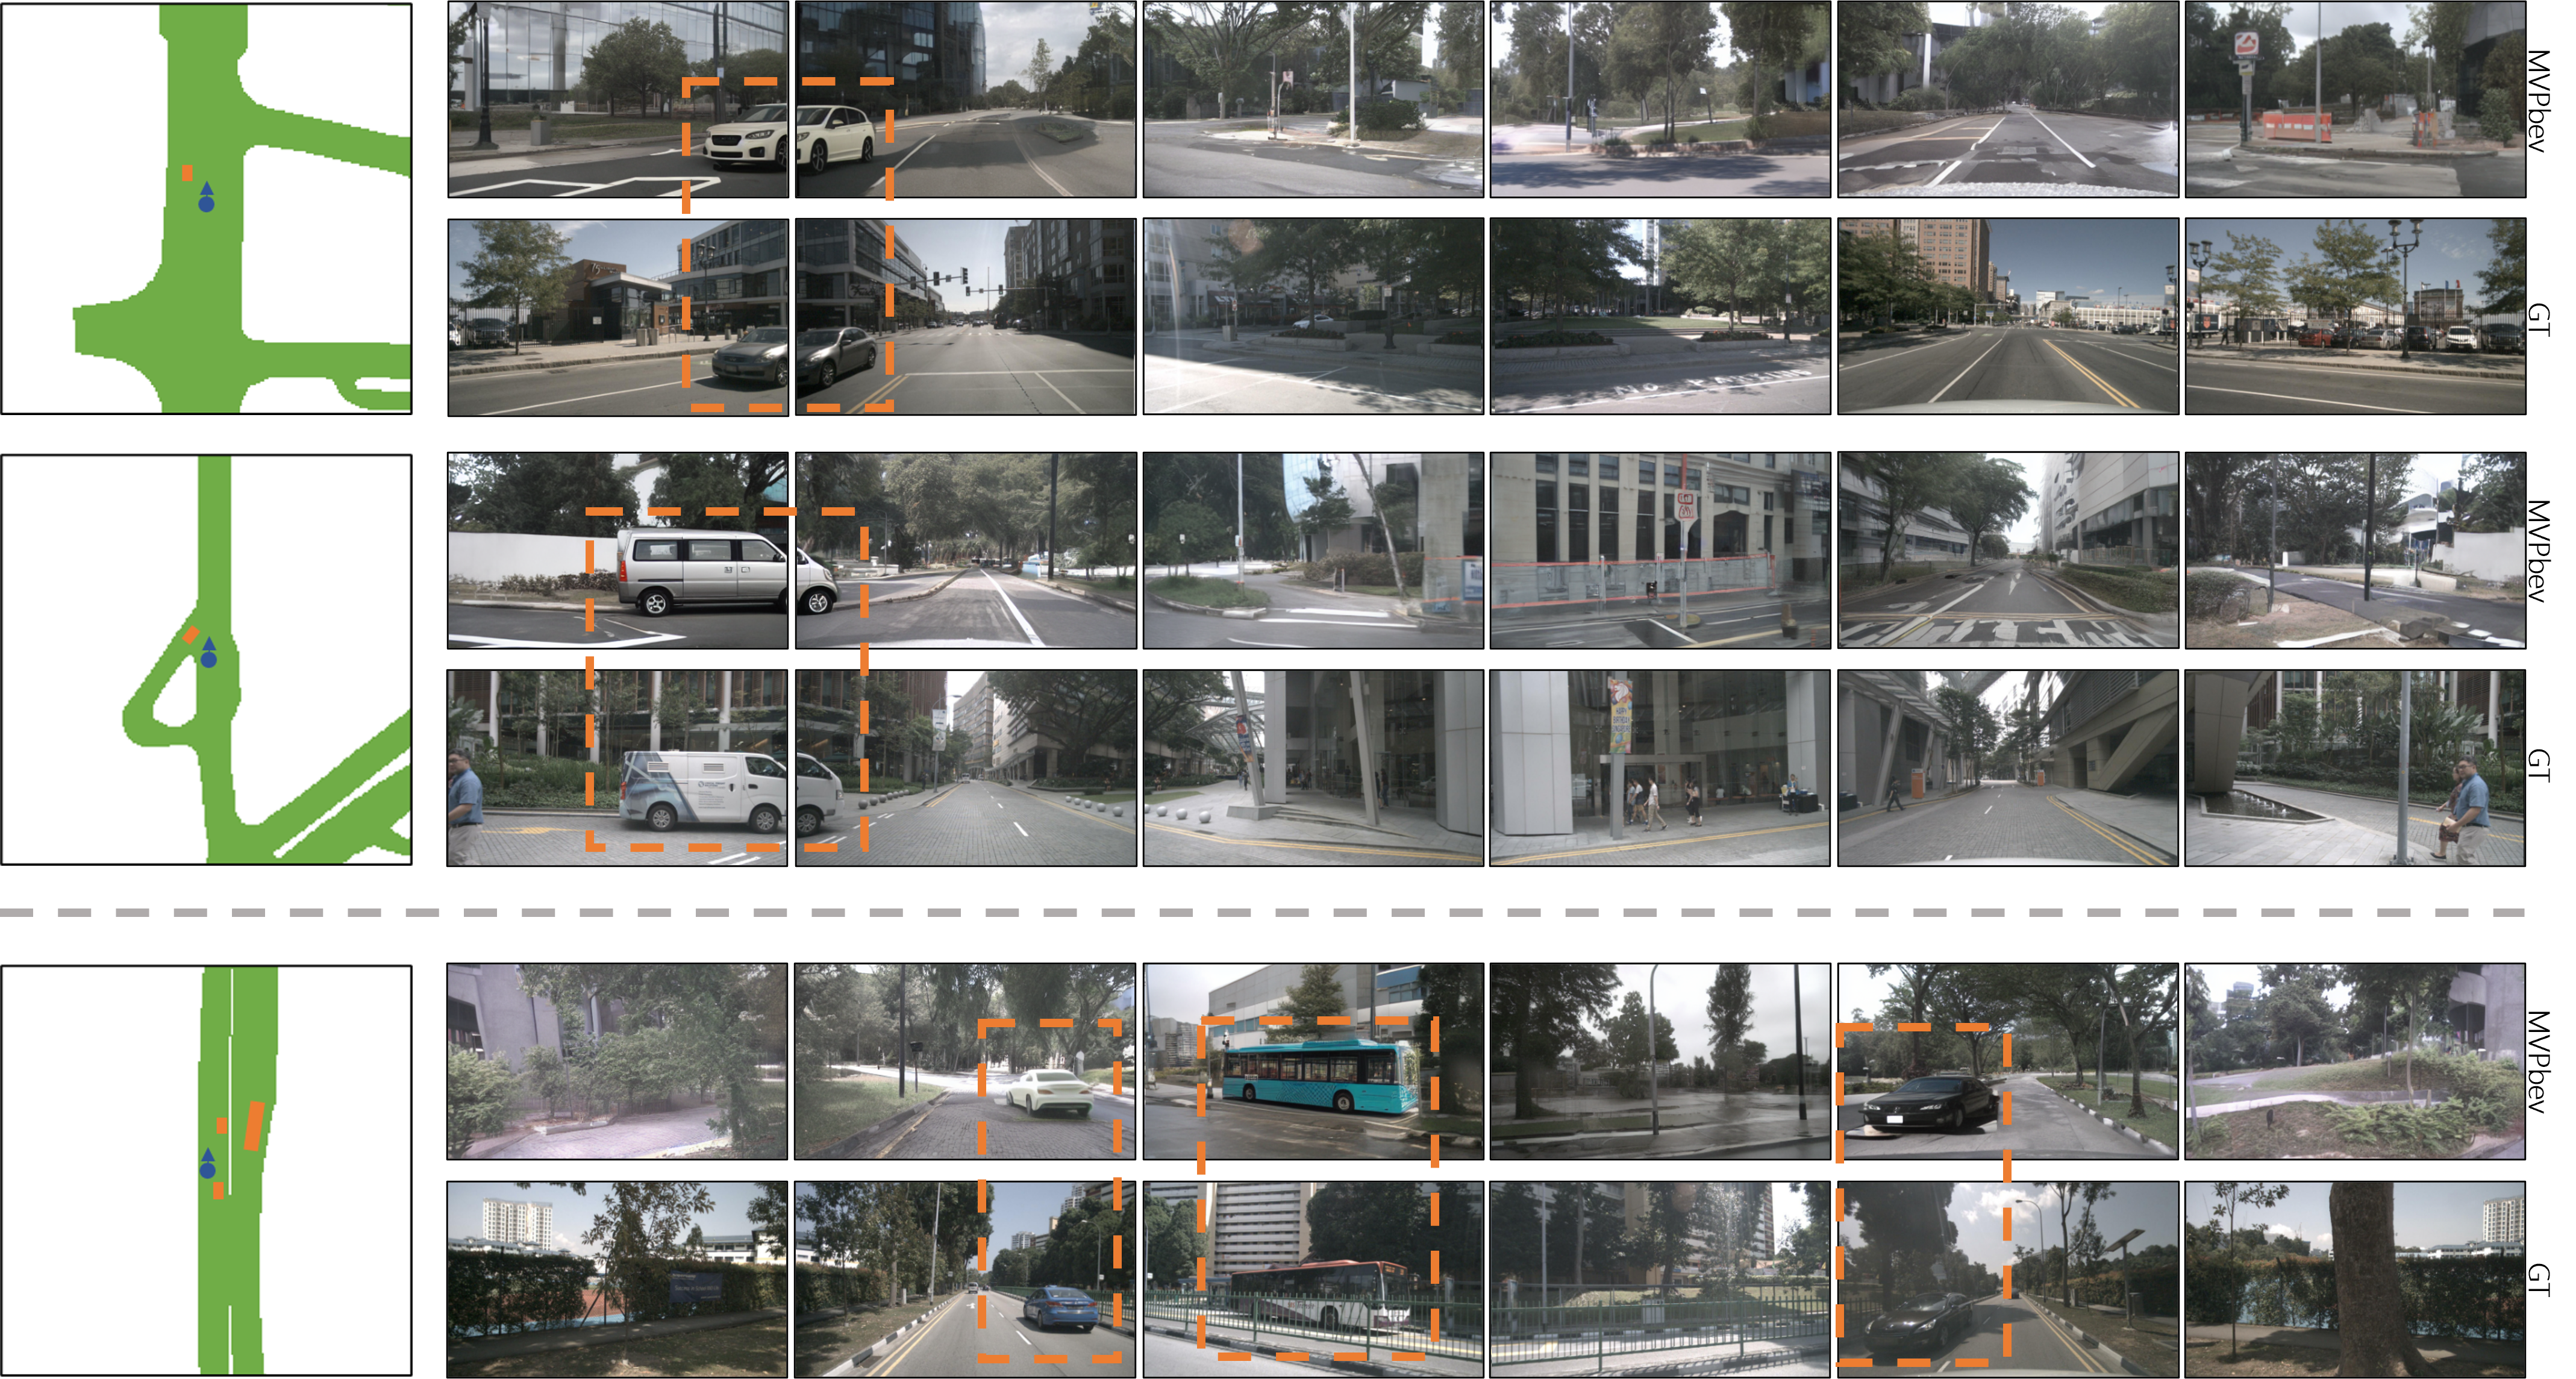
\includegraphics[width=\textwidth]{figures/object_control.png}
\caption{We provide three sets of experiments in this figure. Specifically, the first two sets showcase the multi-view consistency ability of our MVPbev, especially on objects that have been highlighted with orange bounding boxes. The last set of examples demonstrates that MVPbev can be easily applied to multi-object setting.}
\label{fig:object_control}
\end{figure*}


\section{Extension to objects}~\label{sec:obj_details}

Though not shown in the main paper, our MVPbev can be extended to foreground road participants as well. To this end, we assume the 3D object information as well as their visibility are available, together with the original $\textit{B}$. At the projection stage, objects are mapped to 2D perspective view if they are visible. Rather than utilizing the projected 2D bounding boxes in perspective view, we propose to introduce their masks. Specifically, for each object on the validation set of NuScenes, we can find its nearest neighbor in the training set such that their overall distance, which is measured by the averaged relative distances and poses w.r.t. ego car in $L_2$ space, is minimized. We then perform instance-level segmentation on this nearest-neighbor object and obtain its binary mask on $M$ views. These masks are further pasted to $\{S_m\}_{m=1}^M$, leading to an additional semantic class in $c_b$. To effectively leverage the updated $\{S_m\}_m$ at the second stage, we further fine-tune our multi-view LDM with additional control signals.

We provide examples of our extended MVPbev model in Fig.~\ref{fig:object_control}. As can be found in this figure, our MVPbev is able to handle various objects in a cross-view consistent manner.

\section{More qualitative results}~\label{sec:qual_res}
% \textcolor{red}{In this section, we provide more qualitative results of our MVPbev to showcase our comprehensive controllability and generalizability.}

\noindent{\textbf{Qualitative results of MVPbev}} We provide more regular results generated from NuScenes validation set in Fig.~\ref{fig:additional_results}. As can be found in this figure, MVPbev can generate photo-realistic, multi-view consistent, and diverse images from complex road layouts in BEV and text prompts. In addition, we further provide visual examples to demonstrate our controllability over diverse prompts in Fig.\ref{fig:fix_bev_results}. Again, we observe that with the same input BEV semantics while various text prompts as the control signal, our method can generalize to unseen text prompts beyond our training settings in both prompt format and textual semantics.

% seems unnecessary
% \noindent{\textbf{Controlability w.r.t BEV}} \textcolor{red}{In Fig.\ref{??}, we fixed 
% }

% \noindent{\textbf{Prompt controllability results}} \textcolor{red}{In Fig.\ref{??}, we generated several groups of images with input BEV semantics fixed while text prompts vary to show that our method can generalize to unseen text prompts beyond our training settings in both prompt format and textual semantics.}

\noindent{\textbf{View-point generalizability}} Similar to Fig.\textcolor{red}{9} in our main paper, more visual exmaples are provided in Fig.\ref{fig:camera_pose_results} to show how our method generalizes well to different camera setups, which is beyond SOTA MagicDrive~\cite{gao2023magicdrive} that requires far more training samples.

\noindent{\textbf{Instance-level controllability}} Please see Fig.\ref{fig:color_control_results} for more generated instances with its paired text prompts.

% \subsection{Regular results} We provide more regular results generated from NuScenes validation set in Fig.~\ref{fig:additional_results}.
% %prompt fixed, BEV varies 
% \subsection{Controlability w.r.t BEV}
% %BEV fixed, prompt varies 
% \subsection{Controlability w.r.t prompts}
% \subsection{Generalizability w.r.t camera pose}
% \subsection{Instance color control results}

% \textcolor{red}{As can be found in this section, our MVPbev is able to generate photo-realistic images which are visually of similar styles and our generated images are semantically consistent w.r.t. semantic BEV as well as text prompts. Moreover, our method can meet the requirements for multiple instance control.}

\begin{figure*}[h]
\centering
\includegraphics[width=\textwidth]{figures/supplementary/regular_results.jpg}
\caption{We provide five examples from NuScenes validation set. Our MVPbev is able to generate photo-realistic, multi-view consistent, and diverse images from complex road layouts in BEV and text prompts.}
\label{fig:additional_results}
\end{figure*}

\begin{figure*}[h]
\centering
\includegraphics[width=\textwidth]{figures/supplementary/fixed_bev_prompt_contrl.png}
\caption{We provide four generated examples with fixed BEV while text prompt changes. Our MVPbev can generalize to various prompts, yielding diverse results with consistency in both semantic and textual aspect. Notably, our method can even generate results with unseen weather (e.g. "snowy day") that SOTA MagicDrive\cite{gao2023magicdrive} can't achieve (see Conclusion section in their paper).}
\label{fig:fix_bev_results}
\end{figure*}

\begin{figure*}[h]
\centering
\includegraphics[width=\textwidth]{figures/supplementary/camera_pose_results.png}
\caption{We provide three examples that show how our MVPbev generalize to different camera poses. The projected BEV semantics are overlaid in generated results.}
\label{fig:camera_pose_results}
\end{figure*}

\begin{figure*}[]
\centering
\includegraphics[width=\textwidth]{figures/supplementary/color_control_results.jpg}
\caption{We provide more results in instance color control. Our training-free method can handle multiple instance control, ensuring controlled  instances are aligned with their control signals (i.e. multiple instance-level prompts and paired masks), and generate natural instances, integrating well with backgrounds.}
\label{fig:color_control_results}
\end{figure*}
%%
%% The next two lines define the bibliography style to be used, and
%% the bibliography file.
\clearpage

\bibliographystyle{ACM-Reference-Format}
\bibliography{main}


\end{document}
\endinput
%%
%% End of file `sample-authordraft.tex'.
